\begin{problem}{Scroll of Secrets}{standard input}{standard output}{1 second}{512 megabytes}

\textbf{This is an interactive problem}

In the vast kingdom of DataLand, the wise King Algorithmus has hidden a series of magical scrolls along a secret path. Each scroll contains a number, and the scrolls are arranged in strict order, with each successive scroll bearing a larger number than the last. The kingdom's scholars refer to this path as a \textit{singly linked list}, where each scroll not only holds a number but also points to the next scroll in the sequence.

You, the kingdom's chief seeker, have been tasked with finding the first scroll whose number is not less than a magical number $x$, which the king has entrusted to you. The challenge lies in the fact that the path is long, and you may only inspect a limited number of scrolls before the path vanishes into the mists of time.

\begin{center}
  \def \htmlPixelsInCm {45}  % pixels in 1 centimeter in HTML mode
  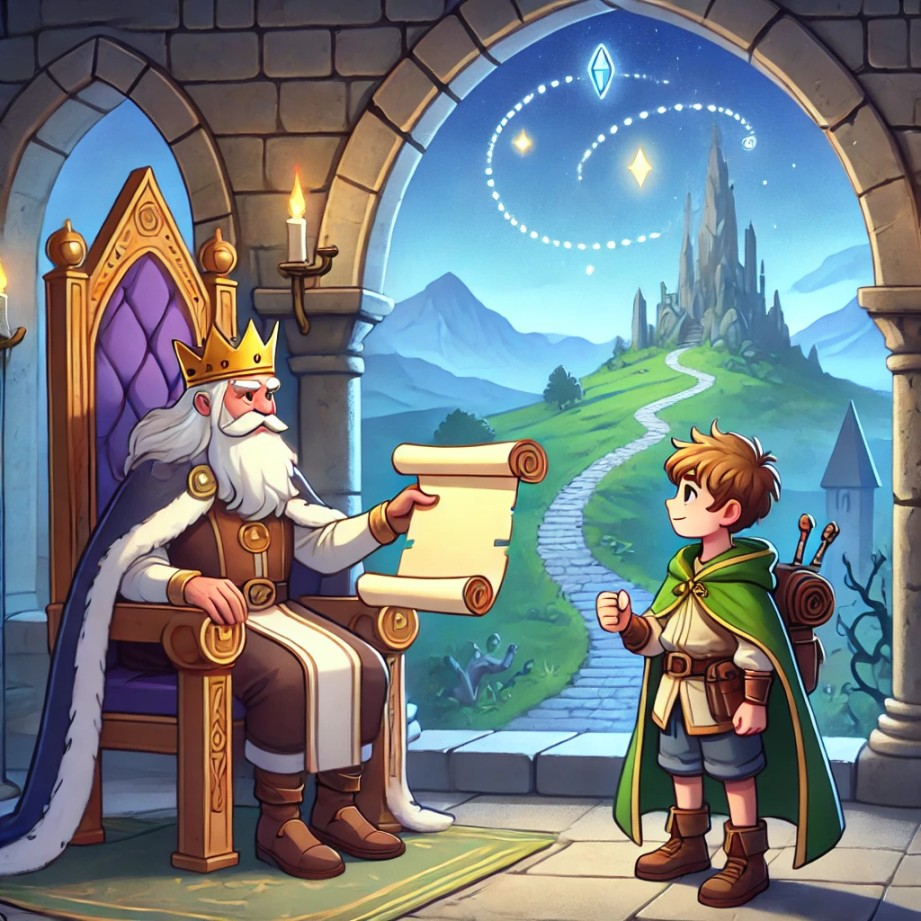
\includegraphics[width=6cm]{scroll.jpg} \\
  \small{The King hands you the magical scroll}
\end{center}

Your mission is to navigate this mysterious path efficiently. Starting from a given scroll, you must determine the smallest number that is greater than or equal to $x$. If no such number exists, you must return to the king with the news that the quest has failed.

\textbf{The Path:}
\begin{itemize}
    \item The path consists of $n$ scrolls, each containing a number and a clue (an index) pointing to the next scroll.
    \item You begin your quest at a scroll indexed as \texttt{start}.
    \item The scrolls are sorted in ascending order, meaning the number on each scroll is less than the number on the next scroll, as long as it exists.
\end{itemize}

\textbf{Your Tools:}
\begin{itemize}
    \item You can ask about a specific scroll by its index to reveal the number it holds and the index of the next scroll.
    \item However, the ancient magic of the path only allows you to ask up to 5000 questions before the path dissolves.
\end{itemize}

You task is to find and report the smallest number on the path that is greater than or equal to $x$. If no such number exists, report that the quest has failed.

\InputFile
The number of scrolls $n$, the index of the first scroll \texttt{start}, and the magical number $x$.

\section*{Constraints}

\begin{itemize}
    \item $1 \leq n \leq 10^5$
    \item $1 \leq \texttt{start} \leq n$
    \item $0 \leq x \leq 10^9$
    \item You may ask no more than 5000 questions.
\end{itemize}

\OutputFile
\begin{itemize}
    \item If you find the desired number, return it to the king. Otherwise, return $-1$ to signify the quest's failure.
\end{itemize}

\Interaction
\begin{itemize}
    \item To make a query about a scroll, print \texttt{? i}, where $i$ is the index of the scroll.
    \item After printing, read two values: \texttt{value\_i}, which is the number on the scroll, and \texttt{next\_i}, which is the index of the next scroll in the sequence.
    \item You may make up to 5000 such queries.
    \item To submit your final answer, print \texttt{! ans}, where \texttt{ans} is the smallest number greater than or equal to $x$. If no such number exists, print \texttt{! -1}.
    \item After the final answer is submitted, your program should terminate.
\end{itemize}

\Scoring
The scoring for this problem depends on the number of queries used:

\begin{itemize}
    \item If you use $\leq 100000$ queries, you will receive 50\% of the points.
    \item If you use $\leq 60000$ queries, you will receive 75\% of the points.
    \item If you successfully use $\leq 5000$ queries, you will receive full points.
\end{itemize}

\Example

\begin{example}
\exmpfile{example.01}{example.01.a}%
\end{example}

\Note
For the first example, in a quest where $n = 5$, \texttt{start = 3}, and $x = 80$, your path may look something like this:
\begin{itemize}
    \item Scroll 1 holds the number 97 and is the last scroll.
    \item Scroll 2 holds the number 58 and points to Scroll 5.
    \item Scroll 3 holds the number 16 and points to Scroll 2.
    \item Scroll 4 holds the number 81 and points to Scroll 1.
    \item Scroll 5 holds the number 79 and points to Scroll 4.
\end{itemize}

A strategy would be to ask 5 queries to get the information for all scrolls, then you would report back to the king with the number 81 as it is the smallest number greater than or equal to 80.

\section*{Hints: }
\begin{itemize}
\item Think about the \textit{nuts and bolts} problem discussed in class. Just as matching each nut to its corresponding bolt required clever strategies, this problem may benefit from a similar approach. Consider using randomization to explore the scrolls efficiently and find the correct number. The key lies in making wise choices about which scrolls to inspect.
\end{itemize}

\end{problem}

